\documentclass[]{article}
\usepackage[T1]{fontenc}
\usepackage[utf8]{inputenc}
\usepackage{lmodern}
\usepackage[a4paper]{geometry}
\usepackage{polski}
\usepackage{tocloft}
\usepackage{fancyhdr}
\usepackage{graphicx}
\usepackage{float}
\usepackage{hyperref}
% opening
\title{Milionerzy - Projekt Politechnika Lubelska}
\author{Mateusz Walo, Igor Kozak, Oskar Wilkos}
\date{}

\begin{document}
	
	% Tytuł dokumentu
	\maketitle
	
	\begin{center}
		
\includegraphics[width=0.35\textwidth]{pl.jpg} 
	\end{center}
	
	% Spis treści
	\tableofcontents
	\newpage
	
	% Nagłówki
	\fancyhf{} % Resetuje domyślny styl nagłówków i stopek
	\fancyhead[L]{\bfseries Milionerzy - Projekt Politechnika Lubelska} % Nagłówek po lewej stronie
	\pagestyle{fancy}
	\renewcommand{\cftsecfont}{\bfseries} % Czcionka sekcji
	\setlength{\cftsecnumwidth}{2.5em} % Odstęp w numerach sekcji
	
	% Sekcja 1
	\section{Ogólny opis aplikacji}
	Aplikacja jest inspirowana popularną grą \emph{„Milionerzy”} i umożliwia użytkownikowi odpowiadanie na pytania quizowe. Gra oferuje dwa koła ratunkowe: „50/50” i „Telefon do przyjaciela”. Rozgrywka kończy się, gdy użytkownik zdobędzie 1000 punktów, co oznacza zwycięstwo. Każda poprawna odpowiedź daje 100 punktów. Po zakończeniu gry, użytkownik może rozpocząć nową rundę. Aby zmienić poziom trudności, należy zamknąć grę i uruchomić ją ponownie.
	
	\newpage
	
\section{Interfejs graficzny}
	
\begin{figure}[H]
	\centering
	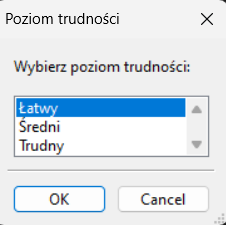
\includegraphics[]{1.png}
	\caption{Wybór poziomu trudności}
	\label{rys:1}
\end{figure}
	
Jak widać na rysunku \ref{rys:1}, użytkownikowi prezentowane jest pierwsze okno aplikacji, w którym dokonuje się wyboru poziomu trudności gry. Interfejs został zaprojektowany tak, aby już na samym początku użytkownik mógł łatwo określić, jak wymagające mają być zadania, z jakimi będzie miał do czynienia. Każdy poziom trudności wiąże się z innym zestawem pytań, co umożliwia indywidualne dostosowanie rozgrywki do umiejętności gracza. Dzięki temu system wyboru poziomu, gra staje się bardziej dostępna – zarówno dla osób szukających mniej wymagającej zabawy, jak i dla tych, którzy pragną zmierzyć się z poważnym wyzwaniem.
	
	\begin{figure}[H]
		\centering
		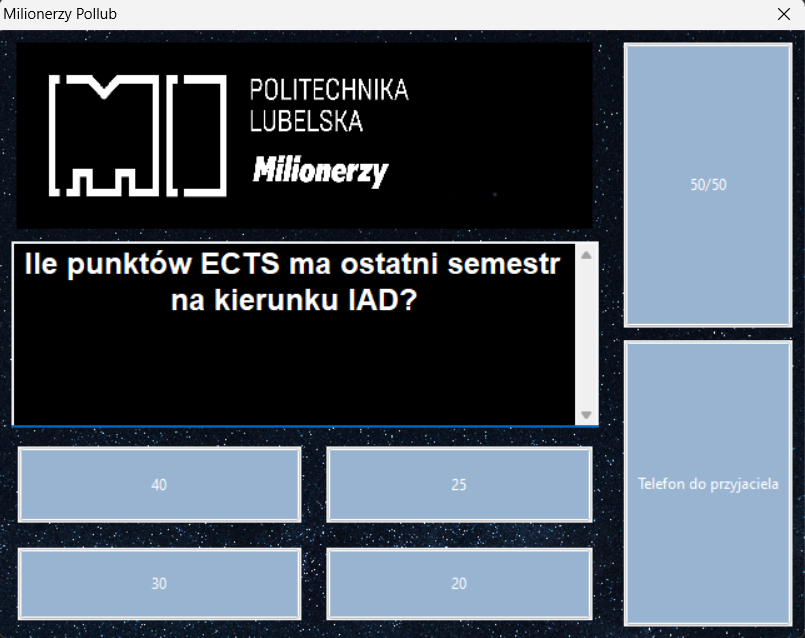
\includegraphics[scale=0.3]{2.png}
		\caption{Interfejs startowy}
		\label{rys:2}
	\end{figure}
Rysunek \ref{rys:2} ilustruje główne okno aplikacji, które pojawia się po wybraniu przez użytkownika odpowiedniego poziomu trudności. W tym widoku widoczne są cztery przyciski odpowiadające możliwym opcjom odpowiedzi, a także obszar z treścią aktualnie zadawanego pytania. Dodatkowo interfejs zawiera dwa elementy reprezentujące koła ratunkowe, które można wykorzystać w krytycznych momentach rozgrywki. Okno to nie tylko prezentuje estetyczny wygląd dzięki funkcji rysowania tła zaimplementowanej w metodzie \texttt{OnPaint}, ale również dynamicznie ładuje i wyświetla pytania poprzez funkcję \texttt{DisplayQuestion}. Dzięki temu rozwiązaniu gra zyskuje na interaktywności i zapewnia płynne przechodzenie między kolejnymi pytaniami. Dodatkowo, dobrze dobrane elementy graficzne i przejrzysty układ pozwalają na intuicyjne poruszanie się po aplikacji, co pozytywnie wpływa na pierwsze wrażenie z użytkowania aplikacji.
	
	\begin{figure}[H]
		\centering
		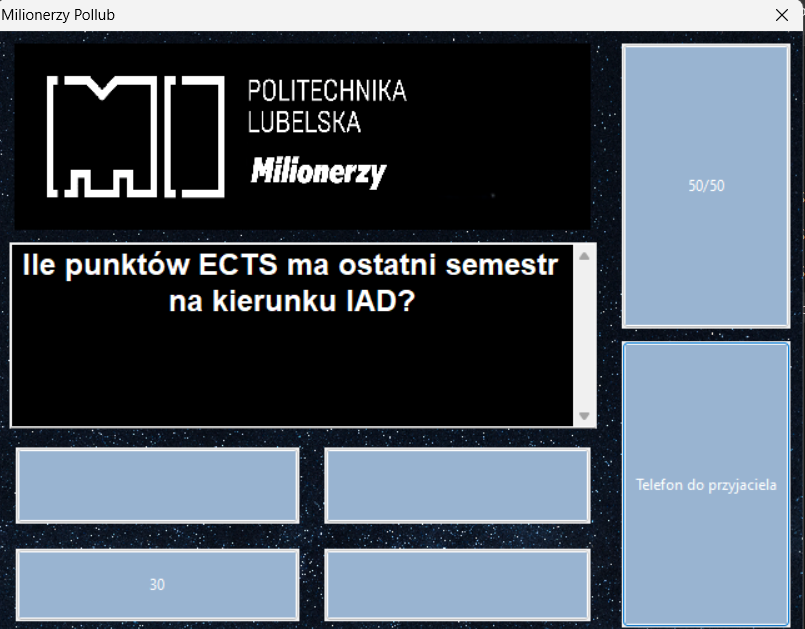
\includegraphics[scale=0.3]{3.png}
		\caption{Koło ratunkowe telefon do przyjaciela}
		\label{rys:3}
	\end{figure}
	Na rysunku \ref{rys:3} przedstawiono moment, w którym użytkownik decyduje się na skorzystanie z koła ratunkowego „Telefon do przyjaciela”. Po aktywacji tego elementu interfejs natychmiast reaguje, usuwając trzy niepoprawne odpowiedzi, co wyraźnie podkreśla istotę udzielanej pomocy. Dzięki takiemu rozwiązaniu, gracz może w krytycznej chwili otrzymać wskazówkę, która umożliwia mu podjęcie lepszej decyzji. Mechanizm ten został zaprojektowany z myślą o zwiększeniu interaktywności gry oraz jej atrakcyjności – możliwość skorzystania z „telefonu” dodaje element strategii, ponieważ gracz musi rozważnie wykorzystać tę szansę, wiedząc, że jest ona dostępna tylko raz w trakcie całej rozgrywki. Wizualne przedstawienie koła ratunkowego oraz natychmiastowa reakcja interfejsu podkreślają dynamikę i intuicyjność działania aplikacji.
	
	\begin{figure}[H]
		\centering
		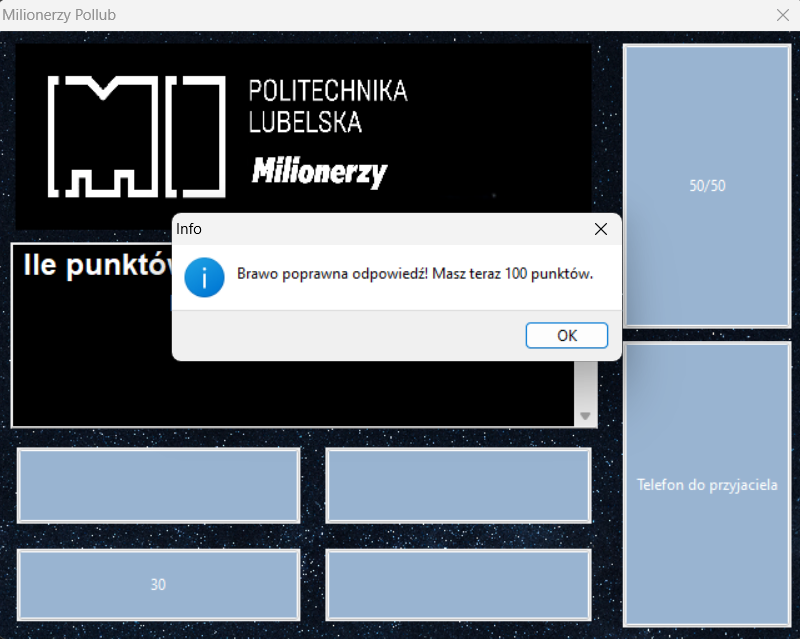
\includegraphics[scale=0.3]{4.png}
		\caption{Wybranie poprawnej odpowiedzi}
		\label{rys:4}
	\end{figure}
Rysunek \ref{rys:4} ukazuje kluczowy moment gry – wybór odpowiedzi przez użytkownika, która okazuje się być prawidłowa. Interfejs graficzny wyraźnie podkreśla zaznaczenie wybranej opcji oraz natychmiast informuje gracza o słuszności jego decyzji. Dodatkowo, system punktacji w czasie rzeczywistym dodaje 100 punktów za każdą poprawną odpowiedź, co jest wizualnie komunikowane w formie okienka informacyjnego. Taki mechanizm nagradzania pozytywnie wpływa na motywację gracza, zachęcając go do kontynuacji rozgrywki. Dbałość o detale w interfejsie – takie jak wyraźne podświetlenie wybranej odpowiedzi i responsywność komunikatów – sprawia, że gra jest nie tylko interaktywna, ale również przyjazna dla użytkownika, co zwiększa ogólne zaangażowanie i satysfakcję z rozgrywki.
	
	\begin{figure}[H]
		\centering
		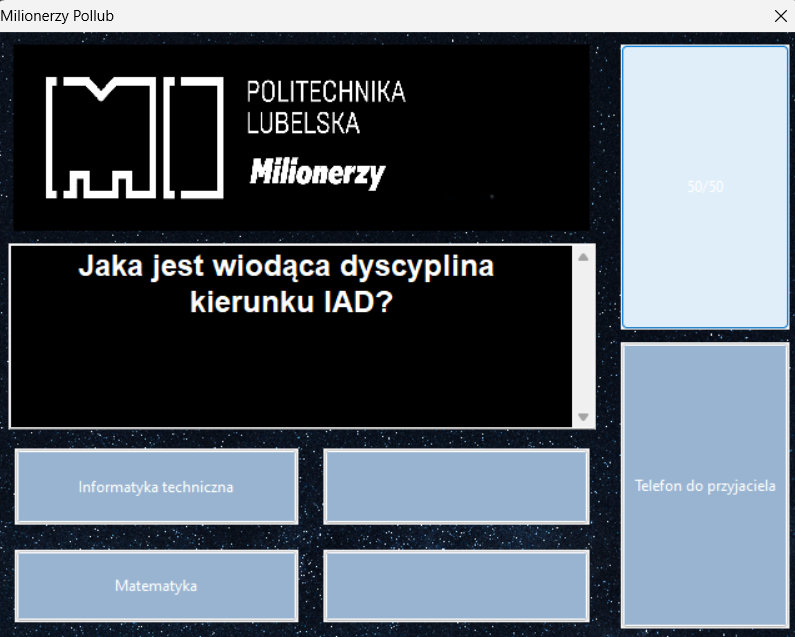
\includegraphics[scale=0.3]{5.png}
		\caption{Koło ratunkowe 50/50}
		\label{rys:5}
	\end{figure}
Na rysunku \ref{rys:5} widać zastosowanie drugiego z dostępnych kół ratunkowych – funkcji 50/50. Po aktywacji tej opcji, interfejs natychmiast usuwa dwie niepoprawne odpowiedzi, pozostawiając użytkownikowi jedynie jedną poprawną oraz jedną potencjalnie mylącą odpowiedź. Takie rozwiązanie znacząco zwiększa szansę na udzielenie właściwej odpowiedzi, szczególnie w sytuacjach, gdy gracz nie jest pewien swojej wiedzy. Wizualna reprezentacja efektu działania koła 50/50 jest intuicyjna – zmiana etykiet przycisków jasno komunikuje, które opcje zostały wyeliminowane. Ponadto, ograniczenie użycia tego koła do jednego razu na grę dodaje strategicznego wymiaru, zmuszając gracza do rozważnego podejmowania decyzji o jego użyciu.
	
	\begin{figure}[H]
		\centering
		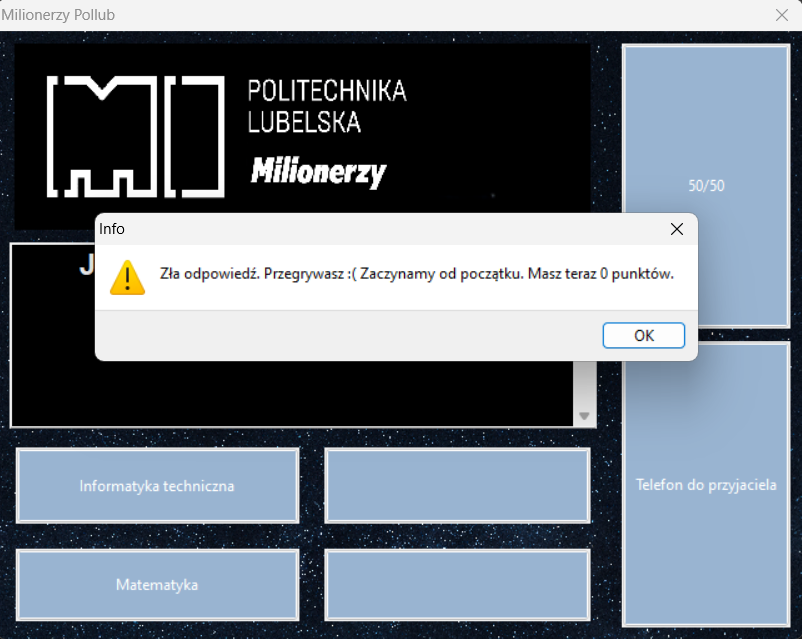
\includegraphics[scale=0.3]{6.png}
		\caption{Komunikat o złej odpowiedzi}
		\label{rys:6}
	\end{figure}
Rysunek \ref{rys:6} przedstawia sytuację, w której gracz udzielił błędnej odpowiedzi. Interfejs aplikacji reaguje natychmiast, wyświetlając komunikat ostrzegawczy, który informuje użytkownika o popełnionym błędzie. W wyniku niepoprawnej decyzji, liczba zdobytych punktów zostaje zresetowana do zera, a gra rozpoczyna się od nowa – ale na tym samym, wybranym wcześniej poziomie trudności. Takie rozwiązanie ma na celu nie tylko zwiększenie realizmu gry, ale również zachęcenie użytkownika do ponownej analizy i lepszego przygotowania się do kolejnych rund. Jasny i czytelny komunikat sprawia, że gracz od razu wie, co poszło nie tak, a sam fakt resetu punktów motywuje do bardziej przemyślanych wyborów w przyszłości.
	
	\begin{figure}[H]
		\centering
		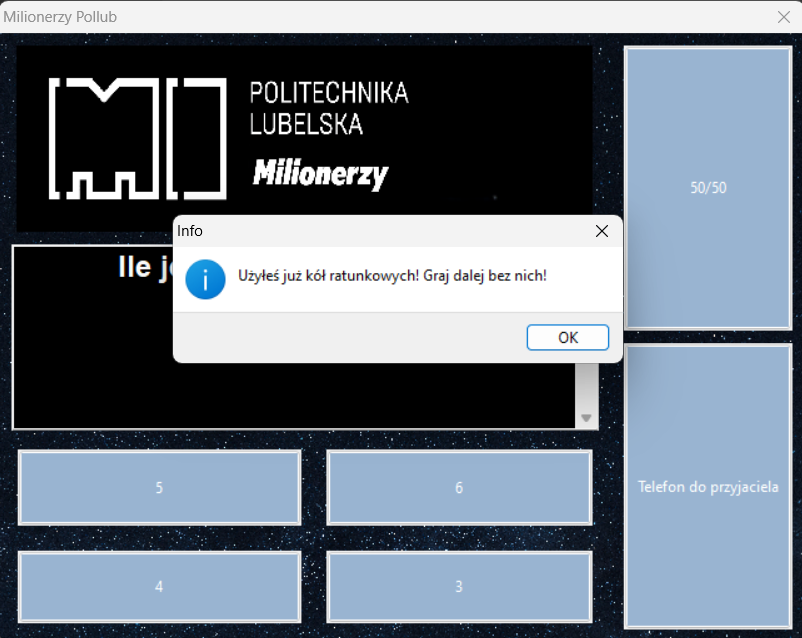
\includegraphics[scale=0.3]{8.png}
		\caption{Komunikat o użyciu kół ratunkowych}
		\label{rys:7}
	\end{figure}
Na rysunku \ref{rys:7} widzimy komunikat, który informuje gracza, iż wszystkie dostępne koła ratunkowe zostały już wykorzystane. Taki komunikat jest niezwykle ważny, ponieważ pełni funkcję informacyjną – użytkownik zostaje ostrzeżony, że nie będzie miał już możliwości skorzystania z dodatkowej pomocy przy rozwiązywaniu pytań. Dzięki temu gracz jest zmuszony do polegania wyłącznie na swojej wiedzy i intuicji w kolejnych etapach gry. Przejrzystość komunikatu oraz jego strategiczne umiejscowienie w interfejsie podkreślają dbałość o szczegóły, co dodatkowo zwiększa realizm i emocjonujący charakter rozgrywki. Informacja ta ma również walor motywacyjny – zmusza do bardziej przemyślanych decyzji, co wpływa na ogólne doświadczenie użytkownika.
	
	\begin{figure}[H]
		\centering
		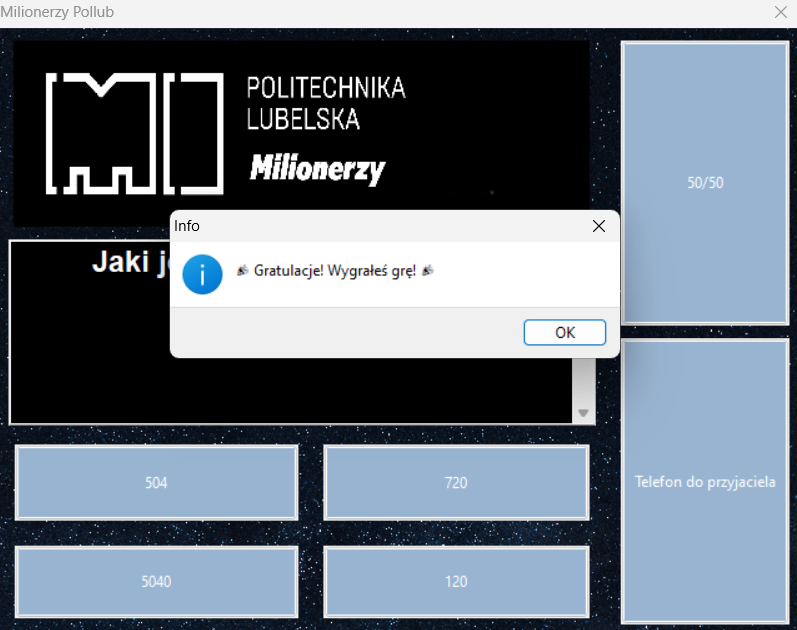
\includegraphics[scale=0.3]{9.png}
		\caption{Komunikat o wygranej}
		\label{rys:8}
	\end{figure}
Rysunek \ref{rys:8} przedstawia finalny moment gry, kiedy gracz osiąga 1000 punktów dzięki serii poprawnych odpowiedzi. Na ekranie pojawia się komunikat gratulacyjny, który nie tylko informuje o zwycięstwie, ale także podkreśla satysfakcję i sukces osiągnięty przez użytkownika. Taki efekt końcowy jest kluczowy, gdyż stanowi nagrodę za wysiłek włożony w grę, a jednocześnie motywuje do powtórzenia rozgrywki lub podejmowania nowych wyzwań. Wizualne elementy komunikatu, takie jak kolory, czcionki i układ, zostały starannie dobrane, aby podkreślić wyjątkowość tego momentu. Dzięki temu użytkownik doświadcza pozytywnych emocji, co wpływa na ogólną atrakcyjność aplikacji i zwiększa jej wartość rozrywkową.

	\section{Struktura kodu}
	
	\subsection{Nagłówki i biblioteki}
	
	Kod rozpoczyna się od dołączenia wymaganych bibliotek oraz plików nagłówkowych. Główne użyte elementy to:
	
	\begin{itemize}
	\item \texttt{\#include "ProjektMain.h"} - Plik nagłówkowy projektu, który zawiera deklaracje klas, funkcji oraz zmiennych specyficznych dla tego projektu. Dzięki temu możliwe jest oddzielenie interfejsu od implementacji oraz łatwiejsze zarządzanie kodem.
	\item \texttt{\#include <wx/msgdlg.h>} - Biblioteka WX Widgets do obsługi okien dialogowych. Umożliwia wyświetlanie komunikatów, ostrzeżeń i informacji, co jest kluczowe dla interaktywności aplikacji oraz komunikacji z użytkownikiem.
	\item \texttt{\#include <nlohmann/json.hpp>} - Biblioteka JSON, która umożliwia łatwe wczytywanie i przetwarzanie danych zapisanych w formacie JSON. Dzięki niej aplikacja może dynamicznie ładować bazę pytań z plików, co zwiększa elastyczność i skalowalność projektu.
	\item \texttt{\#include <random>} - Biblioteka służąca do generowania losowych wartości. Jest wykorzystywana do losowania pytań oraz do mieszania kolejności odpowiedzi, co wprowadza element nieprzewidywalności i urozmaicenia w rozgrywce.
	\item \texttt{\#include <algorithm>} - Biblioteka zawierająca metody i algorytmy, które są używane m.in. do losowego tasowania elementów, co jest kluczowe przy losowym wybieraniu pytań i odpowiedzi.
	\end{itemize}
	
	Struktura \texttt{Question} przechowuje dane pojedynczego pytania quizowego:
	
\begin{itemize}
	\item \texttt{std::string tresc} - Zawiera treść pytania, którą użytkownik widzi na ekranie.
	\item \texttt{std::vector<std::string> odpowiedzi} - Lista możliwych odpowiedzi, z której użytkownik wybiera jedną.
	\item \texttt{std::string poprawna\_odpowiedz} - Przechowuje poprawną odpowiedź, co jest wykorzystywane przy weryfikacji odpowiedzi udzielonej przez gracza.
\end{itemize}
	
	\subsection{Zmienne globalne}
	
	Następnie zdefiniowane są zmienne globalne używane w aplikacji:
	
\begin{itemize}
	\item \texttt{std::vector<Question> questions} - Lista wszystkich pytań dostępnych w bazie. Pozwala na dynamiczne dodawanie lub usuwanie pytań, co ułatwia modyfikację zawartości quizu.
	\item \texttt{std::vector<bool> askedQuestions} - Tablica logiczna, która śledzi, które pytania zostały już zadane. Dzięki temu mechanizmowi unika się powtarzania pytań w jednej sesji gry.
	\item \texttt{size\_t currentQuestionIndex} - Zmienna przechowująca indeks aktualnie wyświetlanego pytania. Umożliwia łatwe odwoływanie się do bieżącego elementu z listy pytań.
	\item \texttt{bool fiftyFiftyUsed, phoneAFriendUsed, fiftyFiftyUsedGlobal, phoneAFriendUsedGlobal} - Flagi służące do monitorowania użycia kół ratunkowych. Rozróżnienie na lokalne i globalne flagi pozwala na precyzyjne kontrolowanie dostępności opcji pomocy w trakcie rozgrywki.
	\item \texttt{int points} - Zmienna przechowująca aktualną liczbę punktów zdobytych przez użytkownika. Mechanizm punktacji jest kluczowy dla oceny postępów gracza oraz określania warunków zwycięstwa.
\end{itemize}
	
	\subsection{Funkcja \texttt{wxbuildinfo}}
	
	Funkcja \texttt{wxbuildinfo} zwraca informacje o kompilacji aplikacji:
	
	\begin{itemize}
		\item Argument \texttt{format} określa, czy zwracane informacje mają być w formacie krótkim, czy długim.
		\item Funkcja wykorzystuje makra preprocesora do dodania informacji o systemie operacyjnym i trybie kompilacji (Unicode/ANSI).
	\end{itemize}
	
	\begin{verbatim}
		wxString wxbuildinfo(wxbuildinfoformat format)
		{
			wxString wxbuild(wxVERSION_STRING);
			
			if (format == long_f)
			{
				#if defined(__WXMSW__)
				wxbuild << _T("-Windows");
				#elif defined(__UNIX__)
				wxbuild << _T("-Linux");
				#endif
				
				#if wxUSE_UNICODE
				wxbuild << _T("-Unicode build");
				#else
				wxbuild << _T("-ANSI build");
				#endif // wxUSE_UNICODE
			}
			
			return wxbuild;
		}
	\end{verbatim}
	
	
	\subsection{Klasa \texttt{ProjektDialog}}
	
	Klasa \texttt{ProjektDialog} reprezentuje główne okno dialogowe aplikacji. To w niej zawarte są wszystkie elementy interfejsu użytkownika oraz logika sterująca rozgrywką.
	
	\subsubsection{Konstruktor i destruktor}
	
	Konstruktor klasy \texttt{ProjektDialog} odpowiada za inicjalizację interfejsu użytkownika oraz załadowanie pytań w oparciu o wybrany przez użytkownika poziom trudności. Inicjalizacja ta obejmuje ustawienie początkowych wartości zmiennych, konfigurację przycisków, pól tekstowych oraz innych elementów interfejsu. Destruktor natomiast jest pusty, co oznacza, że nie wykonuje dodatkowych operacji przy zamykaniu okna – wszystkie zasoby są zarządzane automatycznie lub przez system.
	
	\subsubsection{Metoda \texttt{OnPaint}}
	
	Metoda \texttt{OnPaint} odpowiada za rysowanie tła okna dialogowego. Wykorzystuje obiekt klasy \texttt{wxPaintDC}, który umożliwia rysowanie bezpośrednio na obszarze okna. Kluczowe etapy tej metody to:
	\begin{itemize}
		\item Inicjalizacja obiektu \texttt{wxPaintDC}, co pozwala na wykonywanie operacji graficznych.
		\item Wczytanie bitmapy tła z pliku (w tym przypadku \texttt{"resources/kosmos.jpg"}), co dodaje aplikacji atrakcyjny wygląd.
		\item Konwersja bitmapy na obiekt \texttt{wxImage} i przeskalowanie jej do aktualnego rozmiaru okna, dzięki czemu tło idealnie dopasowuje się do rozmiarów interfejsu.
		\item Rysowanie przeskalowanej bitmapy na oknie, a następnie wywołanie metody \texttt{event.Skip()}, aby umożliwić dalsze przetwarzanie zdarzenia.
	\end{itemize}
	
	\begin{verbatim}
		void ProjektDialog::OnPaint(wxPaintEvent& event)
		{
			wxPaintDC dc(this);
			
			wxBitmap backgroundBitmap(wxT("resources/kosmos.jpg"), wxBITMAP_TYPE_JPEG);
			
			wxImage scaledImage = backgroundBitmap.ConvertToImage();
			scaledImage = scaledImage.Scale(GetSize().GetWidth(), GetSize().GetHeight());
			
			dc.DrawBitmap(wxBitmap(scaledImage), 0, 0, true);
			
			event.Skip();
		}
	\end{verbatim}
	\subsubsection{Metoda \texttt{DisplayQuestion}}

Metoda \texttt{DisplayQuestion} jest odpowiedzialna za wyświetlenie aktualnego pytania oraz możliwych odpowiedzi na ekranie. W jej działaniu można wyróżnić kilka etapów:

\begin{itemize}
	\item Sprawdzenie, czy lista pytań nie jest pusta. Jeśli nie ma żadnych pytań, zostaje wyświetlony komunikat błędu.
	\item Losowe wybranie pytania spośród dostępnych. Do tego celu wykorzystuje się generator liczb losowych, co pozwala na uniknięcie powtórzeń.
	\item Oznaczenie wybranego pytania jako zadane, co zapobiega jego ponownemu wyświetleniu w trakcie jednej rozgrywki.
	\item Losowe tasowanie kolejności odpowiedzi, aby gracz nie mógł zorientować się, która odpowiedź jest poprawna na podstawie pozycji.
	\item Ustawienie treści pytania oraz etykiet przycisków odpowiedzi przy użyciu metod odpowiednich dla kontrolki tekstowej oraz przycisków.
\end{itemize}

	\begin{verbatim}
		void ProjektDialog::DisplayQuestion()
		{
			if (questions.empty())
			{
				wxMessageBox(_("Brak pytań! :( "), _("Error"), wxOK | wxICON_ERROR);
				return;
			}
			
			std::random_device rd;
			std::mt19937 gen(rd());
			std::uniform_int_distribution<> dis(0, questions.size() - 1);
			do {
				currentQuestionIndex = dis(gen);
			} while (askedQuestions[currentQuestionIndex]);
			
			askedQuestions[currentQuestionIndex] = true;
			Question& question = questions[currentQuestionIndex];
			
			std::vector<std::string> shuffledAnswers = question.odpowiedzi;
			
			std::shuffle(shuffledAnswers.begin(), shuffledAnswers.end(), gen);
			
			TextCtrl1->SetValue(wxString::FromUTF8(question.tresc));
			Button1->SetLabel(wxString::FromUTF8(shuffledAnswers[0]));
			Button2->SetLabel(wxString::FromUTF8(shuffledAnswers[1]));
			Button3->SetLabel(wxString::FromUTF8(shuffledAnswers[2]));
			Button4->SetLabel(wxString::FromUTF8(shuffledAnswers[3]));
			
			fiftyFiftyUsed = false;
			phoneAFriendUsed = false;
		}
	\end{verbatim}
	
\subsubsection{Metoda \texttt{LoadQuestionsFromFile}}

Metoda \texttt{LoadQuestionsFromFile} odpowiada za wczytywanie pytań z pliku JSON. Umożliwia to dynamiczne ładowanie bazy pytań w zależności od wybranego poziomu trudności. Jej działanie obejmuje:
\begin{itemize}
	\item Otwarcie pliku z bazą pytań przy użyciu \texttt{std::ifstream}.
	\item Wczytanie danych z pliku do obiektu typu \texttt{json}, co ułatwia późniejsze przetwarzanie danych.
	\item Wyczyść listę dotychczasowych pytań oraz stan zadanych pytań, aby przygotować przestrzeń na nowe dane.
	\item Iterację przez każdy element w sekcji "pytania" w pliku JSON, utworzenie obiektu \texttt{Question} oraz dodanie go do listy pytań.
	\item Jeśli plik nie może zostać otwarty, wyświetlenie komunikatu błędu, co informuje użytkownika o problemie z dostępem do bazy pytań.
\end{itemize}
	
	\begin{verbatim}
		void ProjektDialog::LoadQuestionsFromFile(const wxString& fileName)
		{
			std::ifstream file(fileName.ToStdString());
			if (file.is_open())
			{
				json jsonData;
				file >> jsonData;
				questions.clear();
				askedQuestions.clear();
				for (const auto& item : jsonData["pytania"])
				{
					Question q;
					q.tresc = item["tresc"];
					q.odpowiedzi = item["odpowiedzi"].get<std::vector<std::string>>();
					q.poprawna_odpowiedz = item["poprawna_odpowiedz"];
					questions.push_back(q);
					askedQuestions.push_back(false);
				}
				file.close();
			}
			else
			{
				wxMessageBox(_("Nie można wczytać bazy pytań"), _("Error"), wxOK | wxICON_ERROR);
			}
		}
	\end{verbatim}
	\subsubsection{Metoda \texttt{OnButtonClicked}}

Metoda \texttt{OnButtonClicked} obsługuje interakcję użytkownika z przyciskami odpowiedzi. Odpowiada za weryfikację udzielonej odpowiedzi oraz aktualizację stanu gry:
\begin{itemize}
	\item Pobiera identyfikator klikniętego przycisku oraz jego etykietę.
	\item Za pomocą funkcji \texttt{trimString} usuwa zbędne białe znaki, co zapewnia poprawne porównanie tekstów.
	\item Dokonuje porównania odpowiedzi użytkownika z poprawną odpowiedzią, przy czym ignorowana jest wielkość liter – dzięki temu system jest bardziej przyjazny.
	\item W przypadku udzielenia poprawnej odpowiedzi, metoda zwiększa liczbę punktów oraz wyświetla komunikat potwierdzający sukces. Po osiągnięciu 1000 punktów gra informuje o zwycięstwie, resetując jednocześnie stan gry.
	\item Jeśli odpowiedź jest błędna, liczba punktów jest resetowana do zera, a użytkownik otrzymuje odpowiedni komunikat ostrzegawczy. Dodatkowo resetowany jest stan kół ratunkowych, co umożliwia ponowne rozpoczęcie gry.
\end{itemize}

	\begin{verbatim}
		void ProjektDialog::OnButtonClicked(wxCommandEvent& event)
		{
			int buttonId = event.GetId();
			std::string correctAnswer = trimString(questions[currentQuestionIndex].poprawna_odpowiedz);
			
			wxButton* clickedButton = dynamic_cast<wxButton*>(event.GetEventObject());
			if (clickedButton)
			{
				std::string userAnswer = trimString(clickedButton->GetLabel().ToStdString());
				std::transform(userAnswer.begin(), userAnswer.end(), userAnswer.begin(), ::tolower);
				std::transform(correctAnswer.begin(), correctAnswer.end(), correctAnswer.begin(), ::tolower);
				
				if (userAnswer == correctAnswer)
				{
					points += 100;
					wxMessageBox(wxString::Format(_("Brawo poprawna odpowiedź! Masz teraz %d punktów."), points), _("Info"), wxOK | wxICON_INFORMATION);
					if (points >= 1000)
					{
						wxMessageBox(_("Gratulacje! Wygrałeś grę!"), _("Info"), wxOK | wxICON_INFORMATION);
						points = 0;
						std::fill(askedQuestions.begin(), askedQuestions.end(), false);
					}
					DisplayQuestion();
				}
				else
				{
					points = 0;
					wxMessageBox(wxString::Format(_("Zła odpowiedź. Przegrywasz :( Zaczynamy od początku. Masz teraz %d punktów."), points), _("Info"), wxOK | wxICON_WARNING);
					std::fill(askedQuestions.begin(), askedQuestions.end(), false);
					fiftyFiftyUsedGlobal = false;
					phoneAFriendUsedGlobal = false;
					DisplayQuestion();
				}
			}
		}
	\end{verbatim}
	
	\subsubsection{Metoda \texttt{OnFiftyFifty}}

Metoda \texttt{OnFiftyFifty} obsługuje aktywację koła ratunkowego 50/50, które ma na celu zwiększenie szans gracza na udzielenie poprawnej odpowiedzi poprzez eliminację dwóch błędnych opcji:
\begin{itemize}
	\item Na początku metoda sprawdza, czy już użyto któregokolwiek z kół ratunkowych (50/50 lub Telefon do przyjaciela). Jeśli tak, wyświetlany jest komunikat informacyjny.
	\item Jeśli koło ratunkowe jest dostępne, ustawiane są flagi \texttt{fiftyFiftyUsed} oraz \texttt{fiftyFiftyUsedGlobal} na wartość \texttt{true}, aby zapobiec ponownemu użyciu tego wsparcia.
	\item Metoda pobiera poprawną odpowiedź oraz tworzy listę wszystkich przycisków reprezentujących opcje odpowiedzi.
	\item Następnie, przy użyciu pętli, wyłaniane są przyciski z niepoprawnymi odpowiedziami, które umieszczane są w osobnej liście.
	\item Lista niepoprawnych przycisków jest tasowana przy użyciu generatora liczb losowych, a następnie losowo usuwane są etykiety dwóch z nich, co wizualnie eliminuje te opcje.
\end{itemize}
	\begin{verbatim}
		void ProjektDialog::OnFiftyFifty(wxCommandEvent& event)
		{
			if (fiftyFiftyUsed || fiftyFiftyUsedGlobal || phoneAFriendUsed)
			{
				wxMessageBox(_("Użyłeś już kół ratunkowych! Graj dalej bez nich!"), _("Info"), wxOK | wxICON_INFORMATION);
				return;
			}
			
			fiftyFiftyUsed = true;
			fiftyFiftyUsedGlobal = true;
			
			std::string correctAnswer = questions[currentQuestionIndex].poprawna_odpowiedz;
			std::vector<wxButton*> buttons = {Button1, Button2, Button3, Button4};
			std::vector<wxButton*> incorrectButtons;
			
			for (auto button : buttons)
			{
				if (button->GetLabel().ToStdString() != correctAnswer)
				{
					incorrectButtons.push_back(button);
				}
			}
			
			std::random_device rd;
			std::mt19937 gen(rd());
			std::shuffle(incorrectButtons.begin(), incorrectButtons.end(), gen);
			incorrectButtons[0]->SetLabel("");
			incorrectButtons[1]->SetLabel("");
		}
	\end{verbatim}
\subsubsection{Metoda \texttt{OnPhoneAFriend}}

Metoda \texttt{OnPhoneAFriend} obsługuje kliknięcie przycisku „Telefon do przyjaciela”, które polega na usunięciu trzech błędnych odpowiedzi z ekranu, zwiększając tym samym szansę na poprawne udzielenie odpowiedzi:
\begin{itemize}
	\item Metoda najpierw sprawdza, czy już użyto któregokolwiek z kół ratunkowych – jeżeli tak, wyświetlany jest odpowiedni komunikat informacyjny.
	\item Jeżeli wsparcie jest dostępne, flagi \texttt{phoneAFriendUsed} i \texttt{phoneAFriendUsedGlobal} są ustawiane na \texttt{true}.
	\item Pobierana jest poprawna odpowiedź, a następnie tworzona jest lista przycisków zawierająca wszystkie możliwe opcje.
	\item Lista przycisków jest tasowana losowo, co zapobiega przewidywalności usuwania opcji.
	\item Następnie metoda przechodzi przez przyciski i usuwa etykiety trzech niepoprawnych opcji, co wizualnie eliminuje te odpowiedzi z interfejsu.
\end{itemize}

	
	\begin{verbatim}
		void ProjektDialog::OnPhoneAFriend(wxCommandEvent& event)
		{
			if (phoneAFriendUsed || phoneAFriendUsedGlobal || fiftyFiftyUsed)
			{
				wxMessageBox(_("Użyłeś już kół ratunkowych! Graj dalej bez nich!"), _("Info"), wxOK | wxICON_INFORMATION);
				return;
			}
			
			phoneAFriendUsed = true;
			phoneAFriendUsedGlobal = true;
			
			std::string correctAnswer = questions[currentQuestionIndex].poprawna_odpowiedz;
			std::vector<wxButton*> buttons = {Button1, Button2, Button3, Button4};
			
			std::random_device rd;
			std::mt19937 gen(rd());
			std::shuffle(buttons.begin(), buttons.end(), gen);
			
			int hiddenCount = 0;
			for (auto button : buttons)
			{
				if (button->GetLabel().ToStdString() != correctAnswer && hiddenCount < 3)
				{
					button->SetLabel("");
					hiddenCount++;
				}
			}
		}
	\end{verbatim}
\subsubsection{Metoda \texttt{OnQuit}}

Metoda \texttt{OnQuit} odpowiada za zakończenie działania aplikacji. Jej zadanie polega na zamknięciu głównego okna dialogowego, co skutkuje zakończeniem całego procesu aplikacji:

	
	\begin{verbatim}
		void ProjektDialog::OnQuit(wxCommandEvent& event)
		{
			Close();
		}
	\end{verbatim}
	\begin{itemize}
	\item Wywołanie metody \texttt{Close()} zamyka okno dialogowe, co jest standardowym sposobem kończenia aplikacji w oparciu o WX Widgets.
\end{itemize}
	
	\subsubsection{Metoda \texttt{OnAbout}}
	
Metoda \texttt{OnAbout} służy do wyświetlenia informacji o aplikacji, takich jak wersja, system operacyjny czy tryb kompilacji. Umożliwia to szybkie uzyskanie szczegółowych danych dotyczących środowiska uruchomieniowego:

	
	\begin{verbatim}
		void ProjektDialog::OnAbout(wxCommandEvent& event)
		{
			wxString msg = wxbuildinfo(long_f);
			wxMessageBox(msg, _("Welcome to..."));
		}
	\end{verbatim}
	\begin{itemize}
		\item Funkcja \texttt{wxbuildinfo(long\_f)} pobiera szczegółowe informacje o kompilacji, a następnie te informacje są wyświetlane w oknie dialogowym za pomocą \texttt{wxMessageBox()}.
	\end{itemize}
	
		\subsection{Funkcja \texttt{main}}
	
	Funkcja \texttt{main} jest punktem wejścia do aplikacji. Jej główne zadania to:
	\begin{itemize}
		\item Ustawienie instancji aplikacji WX Widgets, co jest niezbędne do zarządzania cyklem życia aplikacji.
		\item Uruchomienie głównej pętli aplikacji przy użyciu funkcji \texttt{wxEntry()}, która kontroluje wszystkie zdarzenia w aplikacji.
	\end{itemize}
	
	\begin{verbatim}
		int main()
		{
			wxApp::SetInstance(new ProjektApp);
			return wxEntry();
		}
	\end{verbatim}
	\subsection{Dodatkowe metody}
	
	Oprócz głównych metod, klasa \texttt{ProjektDialog} zawiera również metody pomocnicze, które choć puste, mogą zostać wykorzystane w przyszłości do rozszerzenia funkcjonalności aplikacji:
	
	\begin{itemize}
		\item \texttt{OnInit} - Metoda wywoływana podczas tworzenia okna dialogowego. Obecnie jest pusta, ale może zostać rozszerzona o dodatkowe operacje inicjalizacyjne, które powinny zostać wykonane przy starcie aplikacji.
		\begin{verbatim}
			void ProjektDialog::OnInit(wxInitDialogEvent& event)
			{
			}
		\end{verbatim}
		\item \texttt{OnTextCtrl1Text} - Metoda obsługująca zmiany tekstu w polu tekstowym. Chociaż aktualnie nie zawiera logiki, może być użyta w przyszłości do dynamicznej walidacji lub modyfikacji danych wprowadzanych przez użytkownika.
		\begin{verbatim}
			void ProjektDialog::OnTextCtrl1Text(wxCommandEvent& event)
			{
			}
		\end{verbatim}
	\end{itemize}
\newpage
\section{Podział obowiązków}

\subsection{Mateusz Walo}
	\begin{itemize}
		\item Implementacja logiki gry:
		\begin{itemize}
			\item Opracowanie mechanizmu zadawania pytań i sprawdzania odpowiedzi.
			\item Implementacja systemu punktacji oraz warunków wygranej i przegranej.
		\end{itemize}
		\item Funkcje losujące pytania:
		\begin{itemize}
			\item Implementacja funkcji losującej pytania z bazy danych.
			\item Zapewnienie losowego wyboru pytań, z uwzględnieniem, aby nie powtarzały się w jednej grze.
		\end{itemize}
		\item Projektowanie baz pytań na poziom średni i trudny:
		\begin{itemize}
			\item Opracowanie pytań dostosowanych do średniego i trudnego poziomu trudności.
			\item Weryfikacja poprawności pytań i odpowiedzi.
		\end{itemize}
			\item Przygotowanie raportu LaTeXowego:
		\begin{itemize}
			\item Opracowanie dokumentacji technicznej projektu w formacie LaTeX.
			\item Redakcja i formatowanie raportu, w tym spis treści, sekcje techniczne i graficzne.		
		\end{itemize}
			\item Obsługa repozytorium na GitHub:
		\begin{itemize}
			\item W celu ujednolicenia i kontroli wersji projektu.
			\item Obsługa poprawek i wysyłanie commitów po aktualizacjach w celu spójności.
	\end{itemize}
\end{itemize}

\subsection{Igor Kozak}
	\begin{itemize}
		\item Implementacja biblioteki do obsługi plików JSON:
		\begin{itemize}
			\item Integracja biblioteki JSON do odczytu i zapisu danych.
			\item Implementacja funkcji wczytujących pytania z plików JSON do aplikacji.
		\end{itemize}
		\item Zaprojektowanie bazy danych na pierwszy poziom trudności:
		\begin{itemize}
			\item Opracowanie pytań dla poziomu łatwego.
			\item Weryfikacja poprawności pytań i odpowiedzi.
		\end{itemize}
		\item Przygotowanie instalatora:
		\begin{itemize}
			\item Opracowanie skryptu instalacyjnego dla aplikacji.
			\item Testowanie procesu instalacji na różnych systemach operacyjnych.
		\end{itemize}
		\item Zaktualizowanie ikonki:
		\begin{itemize}
			\item Projektowanie nowej ikonki dla aplikacji.
			\item Integracja ikonki z aplikacją.
	\end{itemize}
\end{itemize}

\subsection{Oskar Wilkos}
\begin{itemize}
	\item Zaprojektowanie interfejsu graficznego:
	\begin{itemize}
		\item Opracowanie projektu interfejsu użytkownika (UI).
		\item Implementacja interfejsu przy użyciu biblioteki WX Widgets.
	\end{itemize}
	\item Implementacja okienka dialogowego do wyboru poziomu trudności:
	\begin{itemize}
		\item Opracowanie okienka dialogowego umożliwiającego wybór poziomu trudności.
		\item Integracja okienka z główną logiką gry.
	\end{itemize}
	\item Przygotowanie plików graficznych i struktury projektowej:
	\begin{itemize}
		\item Tworzenie i przygotowanie plików graficznych używanych w aplikacji.
		\item Organizacja struktury katalogów projektu, w tym zasobów graficznych i plików konfiguracyjnych.
	\end{itemize}
\end{itemize}

\section{Podsumowanie}
Aplikacja \emph{Milionerzy} jest w pełni funkcjonalnym quizem inspirowanym popularnym teleturniejem. Dzięki możliwości wyboru poziomu trudności oraz użyciu kół ratunkowych, gra oferuje różnorodne wyzwania dla użytkowników. Implementacja opiera się na bibliotece WX Widgets, co pozwala na tworzenie interaktywnych i atrakcyjnych wizualnie interfejsów użytkownika. Kod jest dobrze zorganizowany i modularny, co ułatwia jego modyfikację i rozszerzenie o nowe funkcje w przyszłości.

\end{document}